\chapter{Cronograma}
\label{cap:06}

\textbf{Obs:} Este capítulo deve ser elaborado e estar contido em trabalhos de graduação para a Validação de Projeto de TCC. Na Avaliação Final de TCC (DEFESA) este capítulo não deve existir, visto que não haverá atividades após a Avaliação Final.

Segue abaixo o cronograma das atividades que serão executadas até a Avaliação Final de TCC.

\textbf{Obs:} Para facilitar, crie o cronograma usando o modelo do Word contido no projeto (imagens/templateCronograma.docx), ou qualquer outro \textit{software}, salve a imagem e atualize o arquivo imagens/cronograma.png.

\FloatBarrier
\begin{figure*}[!htbp]
	\centering
	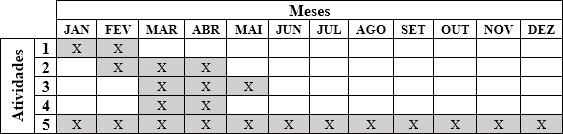
\includegraphics[scale=1]{imagens/cronograma}
\end{figure*}
\FloatBarrier

\begin{enumerate}
	\item Descrição da atividade 1;
	\item Descrição da atividade 2;
	\item Descrição da atividade 3;
	\item Descrição da atividade 4;
	\item Descrição da atividade 5.
\end{enumerate}

